\documentclass{exam}

\usepackage{units} 
\usepackage[fleqn]{amsmath}
\usepackage{float}
\usepackage{mdwlist}
\usepackage{booktabs}
\usepackage{caption}
\usepackage{fullpage}
\usepackage{enumerate}
\usepackage{graphicx}

\usepackage{2in1, lscape} 

\everymath{\displaystyle}

\author{}
\date{January 22, 2014}
\title{Statistics \\ Week One}

\begin{document}

\maketitle
\tableofcontents

  \section{NFL}

  \subsection{Passing Attempts vs. Yards}

  \begin{table}[H]
    \centering
    \begin{tabular}{rrrrr}
      \toprule
      \midrule
         & pa    & py     & pa.scaled & py.scaled \\
      1  & 22.00 & 179.00 & -1.18     & -0.45 \\
      2  & 39.00 & 269.00 & 0.95      & 0.56 \\
      3  & 18.00 & 100.00 & -1.68     & -1.33 \\
      4  & 19.00 & 126.00 & -1.55     & -1.04 \\
      5  & 31.00 & 246.00 & -0.05     & 0.30 \\
      6  & 30.00 & 314.00 & -0.18     & 1.06 \\
      7  & 35.00 & 235.00 & 0.45      & 0.18 \\
      8  & 42.00 & 297.00 & 1.33      & 0.87 \\
      9  & 36.00 & 232.00 & 0.58      & 0.14 \\
      10 & 33.00 & 204.00 & 0.20      & -0.17 \\
      11 & 36.00 & 165.00 & 0.58      & -0.60 \\
      12 & 36.00 & 440.00 & 0.58      & 2.46 \\
      13 & 25.00 & 219.00 & -0.80     & 0.00 \\
      14 & 39.00 & 220.00 & 0.95      & 0.01 \\
      15 & 30.00 & 63.00  & -0.18     & -1.74 \\
      16 & 37.00 & 228.00 & 0.70      & 0.10 \\
      17 & 18.00 & 76.00  & -1.68     & -1.60 \\
      18 & 45.00 & 332.00 & 1.70      & 1.26 \\
      19 & 32.00 & 219.00 & 0.08      & 0.00 \\
      20 & 25.00 & 217.00 & -0.80     & -0.02 \\
      \bottomrule
    \end{tabular}
  \end{table}

  \begin{table}[H]
    \centering
    \begin{tabular}{rlrr}
      \toprule
        & variable & mean & sd \\
      \midrule
      1 & PA       & 36   & 12 \\
      2 & PY       & 267  & 100 \\
      \bottomrule
    \end{tabular}
    \caption{Passing attempts/yards}
  \end{table}

  \begin{figure}[H]
    \centering
    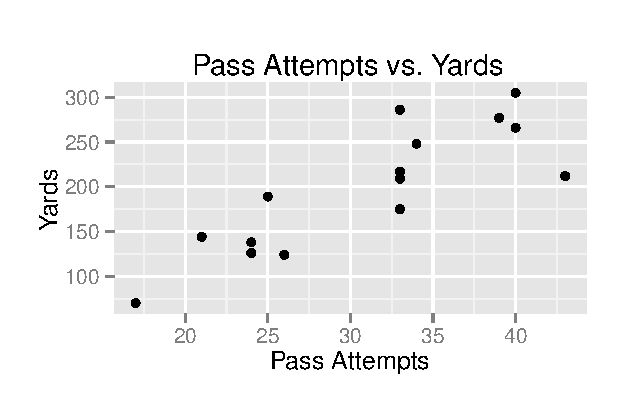
\includegraphics{figures/nfl/passing_attempts_vs_yds.eps}
    \caption{Passing attempts vs. yards}
  \end{figure}

  \[
    c = 0.7225
  \]

  \subsection{Turnover Differential}

  \begin{table}[H]
    \centering
    \begin{tabular}{rrrr}
      \toprule
      GID  & Turnover Differential & Point Differential \\
      \midrule
      3313 & 1                     & 12 \\
      2059 & -3                    & -34 \\
      3444 & 3                     & 10 \\
      1705 & 0                     & 4 \\
      582  & -3                    & 4 \\
      3270 & -1                    & -3 \\
      833  & 2                     & 10 \\
      2700 & 2                     & 14 \\
      1176 & 0                     & 24 \\
      917  & 0                     & -7 \\
      441  & -3                    & 2 \\
      3375 & -1                    & -8 \\
      1156 & 2                     & -10 \\
      1967 & -1                    & -21 \\
      1463 & -1                    & -1 \\
      2660 & 1                     & 13 \\
      1440 & 3                     & 7 \\
      2501 & 6                     & 13 \\
      206  & 4                     & 11 \\
      575  & 2                     & 7 \\
      544  & 0                     & -37 \\
      2888 & 3                     & 3 \\
      3184 & -3                    & -7 \\
      911  & -1                    & -20 \\
      3309 & -2                    & -10 \\
      1218 & 1                     & -10 \\
      852  & -1                    & -6 \\
      3323 & 2                     & 10 \\
      2385 & 3                     & 9 \\
      3094 & -1                    & -18 \\
      2810 & -1                    & -17 \\
      1670 & 2                     & 3 \\
      2926 & -1                    & -2 \\
      2325 & 3                     & 7 \\
      3123 & -2                    & -14 \\
      2642 & 0                     & 4 \\
      2113 & 0                     & -11 \\
      869  & 3                     & 27 \\
      3031 & 4                     & 35 \\
      1715 & 1                     & -1 \\
      \bottomrule
    \end{tabular}
  \end{table}
\end{document}

